\begin{frame}{任务调度流程}

    \scriptsize
    \begin{tikzpicture}[node distance=1.5cm]
        \node (start) [startstop] {Start};
        \node (in) [io, below of=start] {Input: 当前任务 $J$ 所选实例 $I$};
        \node (memory check) [decision, below of=in, yshift=-0.5cm] {$J_m \leqslant I_m$};
        \node (core check) [decision, right of=memory check, xshift=2cm, align=center] {$J_t = Rigid$\\\&\\$J_c > I_c$};
        \node (out of memory) [process, below of=memory check, yshift=-1cm, align=center] {任务调度失败\\$reward = -100$};
        \node (insufficient cores) [process, below of=core check, yshift=-1cm, align=center] {任务调度失败\\$reward = -100$};
        \node (calculate) [process, right of=core check, xshift=2.5cm, align=center] {计算实际执行时间 $T_e$\\加载时间 $T_l$\\写回时间 $T_w$};
        \node (update) [process, right of=calculate, xshift=1.5cm, align=center] {更新实例状态\\更新任务状态};

        \draw [arrow] (start) -- (in);
        \draw [arrow] (in) -- (memory check);
        \draw [arrow] (memory check) -- node[anchor=east] {N} (out of memory);
        \draw [arrow] (memory check) -- node[anchor=south] {Y} (core check);
        \draw [arrow] (core check) -- node[anchor=east] {Y} (insufficient cores);
        \draw [arrow] (core check) -- node[anchor=south] {N} (calculate);
        \draw [arrow] (calculate) -- (update);
    \end{tikzpicture}

\end{frame}

\begin{frame}{任务提交的三种情况}

    \begin{figure}
        \scalebox{1.5}{
            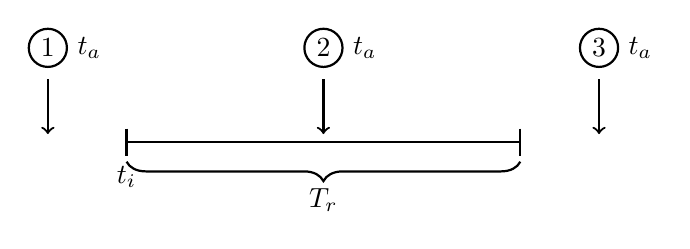
\begin{tikzpicture}[thick]

                \draw[-] (0, 0) -- (5, 0);
                \draw[-] (0, 5pt) -- (0, -5pt) node[below] {$t_i$};
                \draw[-] (5, 5pt) -- (5, -5pt);

                \draw[decorate, decoration={brace, mirror, raise=7pt, amplitude=7pt}] (0, 0) -- (5, 0) node[pos=0.5, below=13pt] {$T_r$};

                \foreach \c/\t in {1/-1, 2/2.5, 3/6} {
                        \draw[->] (\t, 0.8) -- (\t, 3pt);
                        \node[shape=circle,draw,inner sep=2pt] at (\t, 1.2) (char) {\c};
                        \node[right=7] at (\t, 1.2) {$t_a$};
                    }

            \end{tikzpicture}
        }
    \end{figure}

    \begin{enumerate}
        \item 任务在实例空闲之前提交 $t_a \leqslant t_i$
        \item 任务在实例空闲之后、到期之前提交 $t_i < t_a < t_i + T_r$
        \item 任务在实例到期之后提交 $t_a \geqslant t_i + T_r$
    \end{enumerate}

\end{frame}

\begin{frame}{情况一: 任务在实例空闲之前提交 $t_a \leqslant t_i$}{判断是否续租}

    \begin{figure}
        \scalebox{1.5}{
            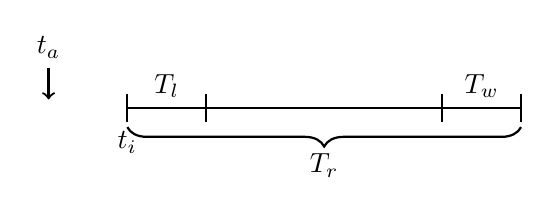
\begin{tikzpicture}[thick]

                \draw[-] (0, 0) -- (5, 0);
                \draw[-] (0, 5pt) -- (0, -5pt) node[below] {$t_i$};
                \draw[-] (5, 5pt) -- (5, -5pt);

                \draw[decorate, decoration={brace, mirror, raise=7pt, amplitude=7pt}] (0, 0) -- (5, 0) node[pos=0.5, below=13pt] {$T_r$};

                \draw[->] (-1, 0.5) node[above] {$t_a$} -- (-1, 3pt);

                \draw[-] (1, 5pt) -- (1, -5pt);
                \node[above] at (0.5, 0) {$T_l$};
                \draw[-] (4, 5pt) -- (4, -5pt);
                \node[above] at (4.5, 0) {$T_w$};

            \end{tikzpicture}
        }
    \end{figure}

    \centering
    \begin{minipage}{0.6\textwidth}
        \IncMargin{1.5em}
        \begin{algorithm}[H]
            $\text{cost} \leftarrow 0$\;
            \While{$T_r - T_l - T_w \leqslant 0$}{
                $T_r \leftarrow T_r + 1$\tcc*{续租一小时}
                $\text{cost} \leftarrow \text{cost} + t_i \text{时刻的实例价格}$\;
            }
        \end{algorithm}
    \end{minipage}

\end{frame}

\begin{frame}{情况一: 任务在实例空闲之前提交 $t_a \leqslant t_i$}{任务能够全部执行 $T_e \leqslant T_r - T_l$}
    \begin{columns}

        \column{0.5\textwidth}

        \begin{figure}
            \scalebox{1.1}{
                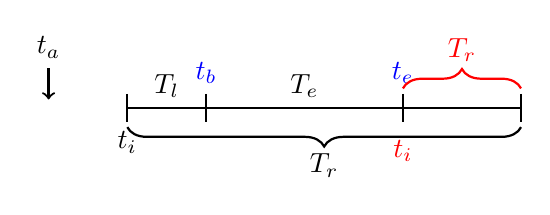
\begin{tikzpicture}[thick]

                    \draw[-] (0, 0) -- (5, 0);
                    \draw[-] (0, 5pt) -- (0, -5pt) node[below] {$t_i$};
                    \draw[-] (5, 5pt) -- (5, -5pt);

                    \draw[decorate, decoration={brace, mirror, raise=7pt, amplitude=7pt}] (0, 0) -- (5, 0) node[pos=0.5, below=13pt] {$T_r$};

                    \draw[->] (-1, 0.5) node[above] {$t_a$} -- (-1, 3pt);

                    \draw[-] (1, 5pt) -- (1, -5pt);
                    \uncover<2->{\node[above] at (1, 5pt) {\textcolor{blue}{$t_b$}};}
                    \node[above] at (0.5, 0) {$T_l$};
                    \draw[-] (3.5, 5pt) -- (3.5, -5pt);
                    \uncover<2->{\node[above] at (3.5, 5pt) {\textcolor{blue}{$t_e$}};}
                    \node[above] at (2.25, 0) {$T_e$};

                    \uncover<3->{
                        \node[below=3] at (3.5, -5pt) {\textcolor{red}{$t_i$}};
                        \draw[red, decorate, decoration={brace, raise=7pt, amplitude=7pt}] (3.5, 0) -- (5, 0) node[pos=0.5, above=13pt] {\textcolor{red}{$T_r$}};
                    }
                \end{tikzpicture}
            }
        \end{figure}

        \column{0.5\textwidth}

        \uncover<2->{任务在 \textcolor{blue}{$t_b = t_i + T_l$} 时刻开始执行, 在 \textcolor{blue}{$t_e = t_b + T_e$} 时刻结束执行.}

        \uncover<3->{
            更新实例状态:
            \begin{itemize}
                \item 实例剩余租期 $\textcolor{red}{T_r} \leftarrow T_r - T_l - T_e$
                \item 实例空闲的时刻 $\textcolor{red}{t_i} \leftarrow \textcolor{blue}{t_e}$
            \end{itemize}
        }

        \uncover<4->{
            更新任务状态:
            \begin{itemize}
                \item 任务长度 $J_l \leftarrow 0$
                \item 任务上一次执行所在的区域 $J_r \leftarrow I_r$
            \end{itemize}
        }

    \end{columns}
\end{frame}

\begin{frame}{情况一: 任务在实例空闲之前提交 $t_a \leqslant t_i$}{任务只能部分执行 $T_e > T_r - T_l$}
    \begin{columns}

        \column{0.5\textwidth}

        \begin{figure}
            \scalebox{1.1}{
                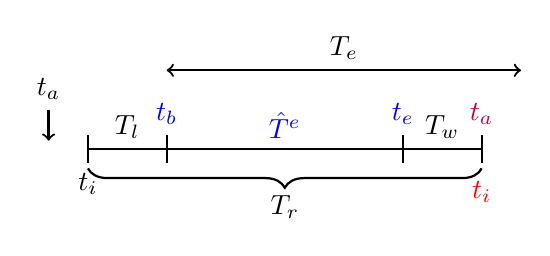
\begin{tikzpicture}[thick]

                    \draw[-] (0, 0) -- (5, 0);
                    \draw[-] (0, 5pt) -- (0, -5pt) node[below] {$t_i$};
                    \draw[-] (5, 5pt) -- (5, -5pt);

                    \draw[decorate, decoration={brace, mirror, raise=7pt, amplitude=7pt}] (0, 0) -- (5, 0) node[pos=0.5, below=13pt] {$T_r$};

                    \draw[->] (-0.5, 0.5) node[above] {$t_a$} -- (-0.5, 3pt);

                    \draw[<->] (1, 1) -- (5.5, 1);
                    \node[above] at (3.25, 1) {$T_e$};

                    \draw[-] (1, 5pt) -- (1, -5pt);
                    \uncover<2->{\node[above] at (1, 5pt) {\textcolor{blue}{$t_b$}};}
                    \node[above] at (0.5, 0) {$T_l$};
                    \draw[-] (4, 5pt) -- (4, -5pt);
                    \uncover<2->{\node[above] at (4, 5pt) {\textcolor{blue}{$t_e$}};}
                    \node[above] at (4.5, 0) {$T_w$};
                    \uncover<2->{\node[above] at (2.5, 0) {\textcolor{blue}{$\hat{T}^e$}};}

                    \uncover<3->{
                        \node[below=3] at (5, -5pt) {\textcolor{red}{$t_i$}};
                    }
                    \uncover<4->{
                        \node[above] at (5, 5pt) {\textcolor{purple}{$t_a$}};
                    }
                \end{tikzpicture}
            }
        \end{figure}

        \column{0.5\textwidth}

        \uncover<2->{任务在 \textcolor{blue}{$t_b = t_i + T_l$} 时刻开始执行, 在 \textcolor{blue}{$t_e = t_i + T_r - T_w$} 时刻结束执行.\\任务实际执行时长 \textcolor{blue}{$\hat{T}^e = t_e - t_b$}.}

        \uncover<3->{
            更新实例状态:
            \begin{itemize}
                \item 实例剩余租期 $\textcolor{red}{T_r} \leftarrow 0$
                \item 实例空闲的时刻 $\textcolor{red}{t_i} \leftarrow t_i + T_r$
            \end{itemize}
        }

        \uncover<4->{
            更新任务状态:
            \begin{itemize}
                \item 任务长度 $J_l \leftarrow \begin{cases}
                              J_l - \hat{T}^e,                           & J_t = \text{Rigid},    \\
                              J_l - \hat{T}^e / \frac{SU(J_c)}{SU(I_c)}, & J_t = \text{Moldable}.
                          \end{cases}$
                \item 任务上一次执行所在的区域 $J_r \leftarrow I_r$
                \item 任务提交时刻 $\textcolor{purple}{t_a} \leftarrow \textcolor{red}{t_i}$
            \end{itemize}
        }

    \end{columns}
\end{frame}

\begin{frame}{情况二: 任务在实例空闲之后、到期之前提交\\$t_i < t_a < t_i + T_r$}
    \begin{columns}

        \column{0.5\textwidth}

        \begin{figure}
            \scalebox{1.1}{
                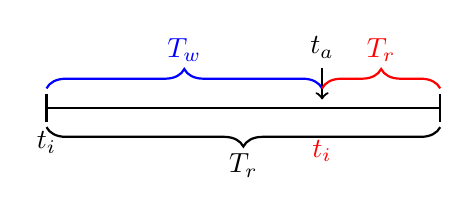
\begin{tikzpicture}[thick]

                    \draw[-] (0, 0) -- (5, 0);
                    \draw[-] (0, 5pt) -- (0, -5pt) node[below] {$t_i$};
                    \draw[-] (5, 5pt) -- (5, -5pt);

                    \draw[decorate, decoration={brace, mirror, raise=7pt, amplitude=7pt}] (0, 0) -- (5, 0) node[pos=0.5, below=13pt] {$T_r$};

                    \draw[->] (3.5, 0.5) node[above] {$t_a$} -- (3.5, 3pt);

                    \uncover<2->{
                        \draw[blue, decorate, decoration={brace, raise=7pt, amplitude=7pt}] (0, 0) -- (3.5, 0) node[pos=0.5, above=13pt] {\textcolor{blue}{$T_w$}};
                    }

                    \uncover<3->{
                        \node[below=3] at (3.5, -5pt) {\textcolor{red}{$t_i$}};
                        \draw[red, decorate, decoration={brace, raise=7pt, amplitude=7pt}] (3.5, 0) -- (5, 0) node[pos=0.5, above=13pt] {\textcolor{red}{$T_r$}};
                    }

                \end{tikzpicture}
            }
        \end{figure}

        \column{0.5\textwidth}

        \uncover<2->{浪费时间 $\textcolor{blue}{T_w} = t_a - t_i$.}

        \uncover<3->{
            更新实例状态:
            \begin{itemize}
                \item 实例剩余租期 $\textcolor{red}{T_r} \leftarrow T_r - \textcolor{blue}{T_w}$
                \item 实例空闲的时刻 $\textcolor{red}{t_i} \leftarrow t_a$
            \end{itemize}
        }

        \uncover<4->{转换为情况一.}

    \end{columns}
\end{frame}

\begin{frame}{情况三: 任务在实例到期之后提交 $t_a \geqslant t_i + T_r$}
    \begin{columns}

        \column{0.5\textwidth}

        \begin{figure}
            \scalebox{1.1}{
                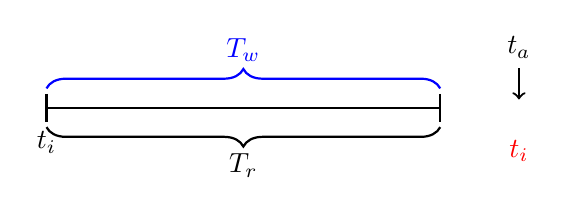
\begin{tikzpicture}[thick]

                    \draw[-] (0, 0) -- (5, 0);
                    \draw[-] (0, 5pt) -- (0, -5pt) node[below] {$t_i$};
                    \draw[-] (5, 5pt) -- (5, -5pt);

                    \draw[decorate, decoration={brace, mirror, raise=7pt, amplitude=7pt}] (0, 0) -- (5, 0) node[pos=0.5, below=13pt] {$T_r$};

                    \draw[->] (6, 0.5) node[above] {$t_a$} -- (6, 3pt);

                    \uncover<2->{
                        \draw[blue, decorate, decoration={brace, raise=7pt, amplitude=7pt}] (0, 0) -- (5, 0) node[pos=0.5, above=13pt] {\textcolor{blue}{$T_w$}};
                    }

                    \uncover<3->{
                        \node[below=3] at (6, -5pt) {\textcolor{red}{$t_i$}};
                    }

                \end{tikzpicture}
            }
        \end{figure}

        \column{0.5\textwidth}

        \uncover<2->{浪费时间 $\textcolor{blue}{T_w} = T_r$.}

        \uncover<3->{
            更新实例状态:
            \begin{itemize}
                \item 实例剩余租期 $\textcolor{red}{T_r} \leftarrow 0$
                \item 实例空闲的时刻 $\textcolor{red}{t_i} \leftarrow t_a$
            \end{itemize}
        }

        \uncover<4->{转换为情况一.}

    \end{columns}
\end{frame}

\begin{frame}{任务调度成功时的奖励}

    \begin{equation*}
        reward = \max \left\{ - (\xi \cdot \text{cost} + \eta \cdot T_w) \cdot \frac{t_e - t_a}{t_e - t_b}, -50 \right\}
    \end{equation*}

    将租金cost和浪费的时间 $T_w$ 作为惩罚项, 任务响应比 $(t_e - t_a)/(t_e - t_b)$ 作为系数. 限制任务调度成功时的奖励不低于 $-50$, 与任务调度失败的奖励 $-100$ 拉开差距.

    其中, $\xi$ 和 $\eta$ 是超参数.

\end{frame}
